% !TEX root = Calli.tex
% Kapitelvorlage

\section{Einleitung}
\label{sec:Einleitung}

Die Anforderungen an die Qualität industriell gefertigter Endprodukte werden immer höher. Um die Kosten der Endkontrolle möglichst gering zu halten, wird eine fehlerresistente und automatisierte Prüfung angestrebt. In vielen Fällen werden dazu Industriekameras eingesetzt. Mit einer angepassten Beleuchtung, der entsprechenden Ausrichtung und einer ausgereiften Software ersetzen sie mittlerweile viele manuelle Kontrollen. Insbesondere zur Farb- und Formerkennung sind sie gut geeignet.

Das bearbeitete Thema hat zum Gegenstand eine Farb- und Formerkennung mit einer Kamera zu realisieren. Grundlage ist das Reaktionsspiel Halli Galli. 

\begin{figure}[H]
    \centering
    \includegraphics[width=7cm]{Abbildungen/cover}
    \caption[Cocer]{Halli Galli - Spielcover}
    \label{fig:Cover}
\end{figure}

\subsection{Halli Galli}

Halli Galli ist ein Reaktionskartenspiel für Kinder. Obwohl das Spielprinzip sehr einfach ist, ist es aufgrund der hohen Spielgeschwindigkeit, der geforderten Konzentrationsfähigkeit sowie der Stressresistenz auch bei vielen Erwachsenen beliebt. 

\textbf{Ziel des Spiels}

Ziel ist es in den Besitz aller Spielkarten zu kommen. Ist dies nicht möglich, gewinnt der Spieler mit den meisten Karten. Hat ein Spieler alle Karten verloren, scheidet er aus. 



\begin{figure}[H]
    \centering
    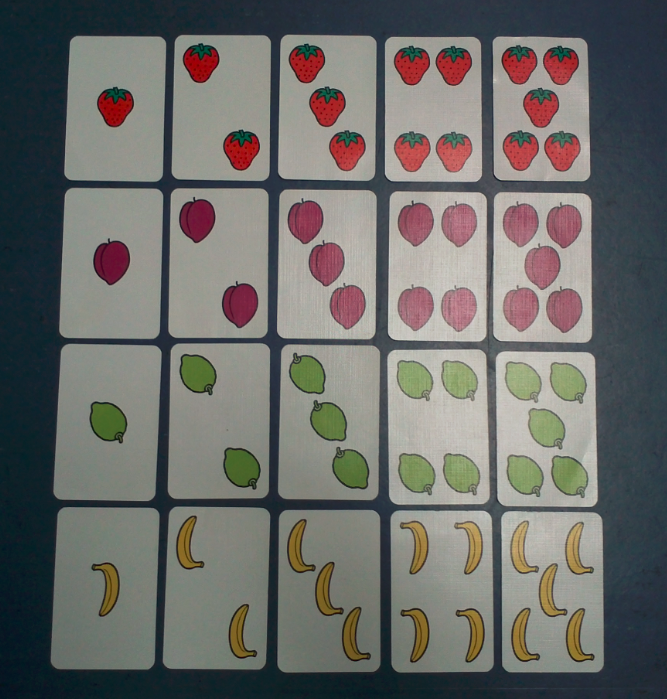
\includegraphics[width=8cm]{Abbildungen/Kartenset}
    \caption[Cocer]{Halli Galli - Kartenset}
    \label{fig:Kartenset}
\end{figure}
\textbf{Spielanleitung}

Alle 56 Fruchtkarten des Kartensets, siehe Abbildung \ref{fig:Kartenset}, werden gleichmäßig an die Mitspieler verteilt. Reihum decken die Spieler die Karten von ihrem Zugstapel auf und legen sie vor sich auf einen separaten Ablagestabel ab. Nach jedem Zug müssen die Früchte auf den offenen Karten gezählt werden. Entspricht die Anzahl einer Sorte genau fünf, so darf auf die Glocke geschlagen werden. Der erste der die Glocke betätigt darf alle offenen Karten einsammeln und unter seinen Zugstapel leben. Reagiert ein Spieler falsch, so muss er jedem Mitspieler eine Karte von seinem Zugstapel geben. 

\subsection{Aufgabenstellung}

Ziel der Projektarbeit ist es mit einer Kamera ein simuliertes Halli Galli Spielfeld von vier Spielern von oben zu filmen. Die Kamera erkennt die Früchte auf den Karten und gibt über eine Bildschirmausgabe an, wenn fünf Früchte einer Sorte erkannt wurden. Abgebildet werden Limonen, Erdbeeren, Pflaumen und Bananen. Schwierigkeiten entstehen durch die zum Teil sehr ähnlichen Farben und Formen der Früchte.

\subsection{Aufbau}

Abbildung~\ref{fig:Anlage} zeigt den benutzten Aufbau zur Erfassung des Spielstandes. Eine Webcam mit USB~-~Schnittstelle wird mit Hilfe eines Aluprofils 40 cm über dem Spielaufbau positioniert.

%Abbildung Aufbau / Kamera
\begin{figure}[]
    \centering
    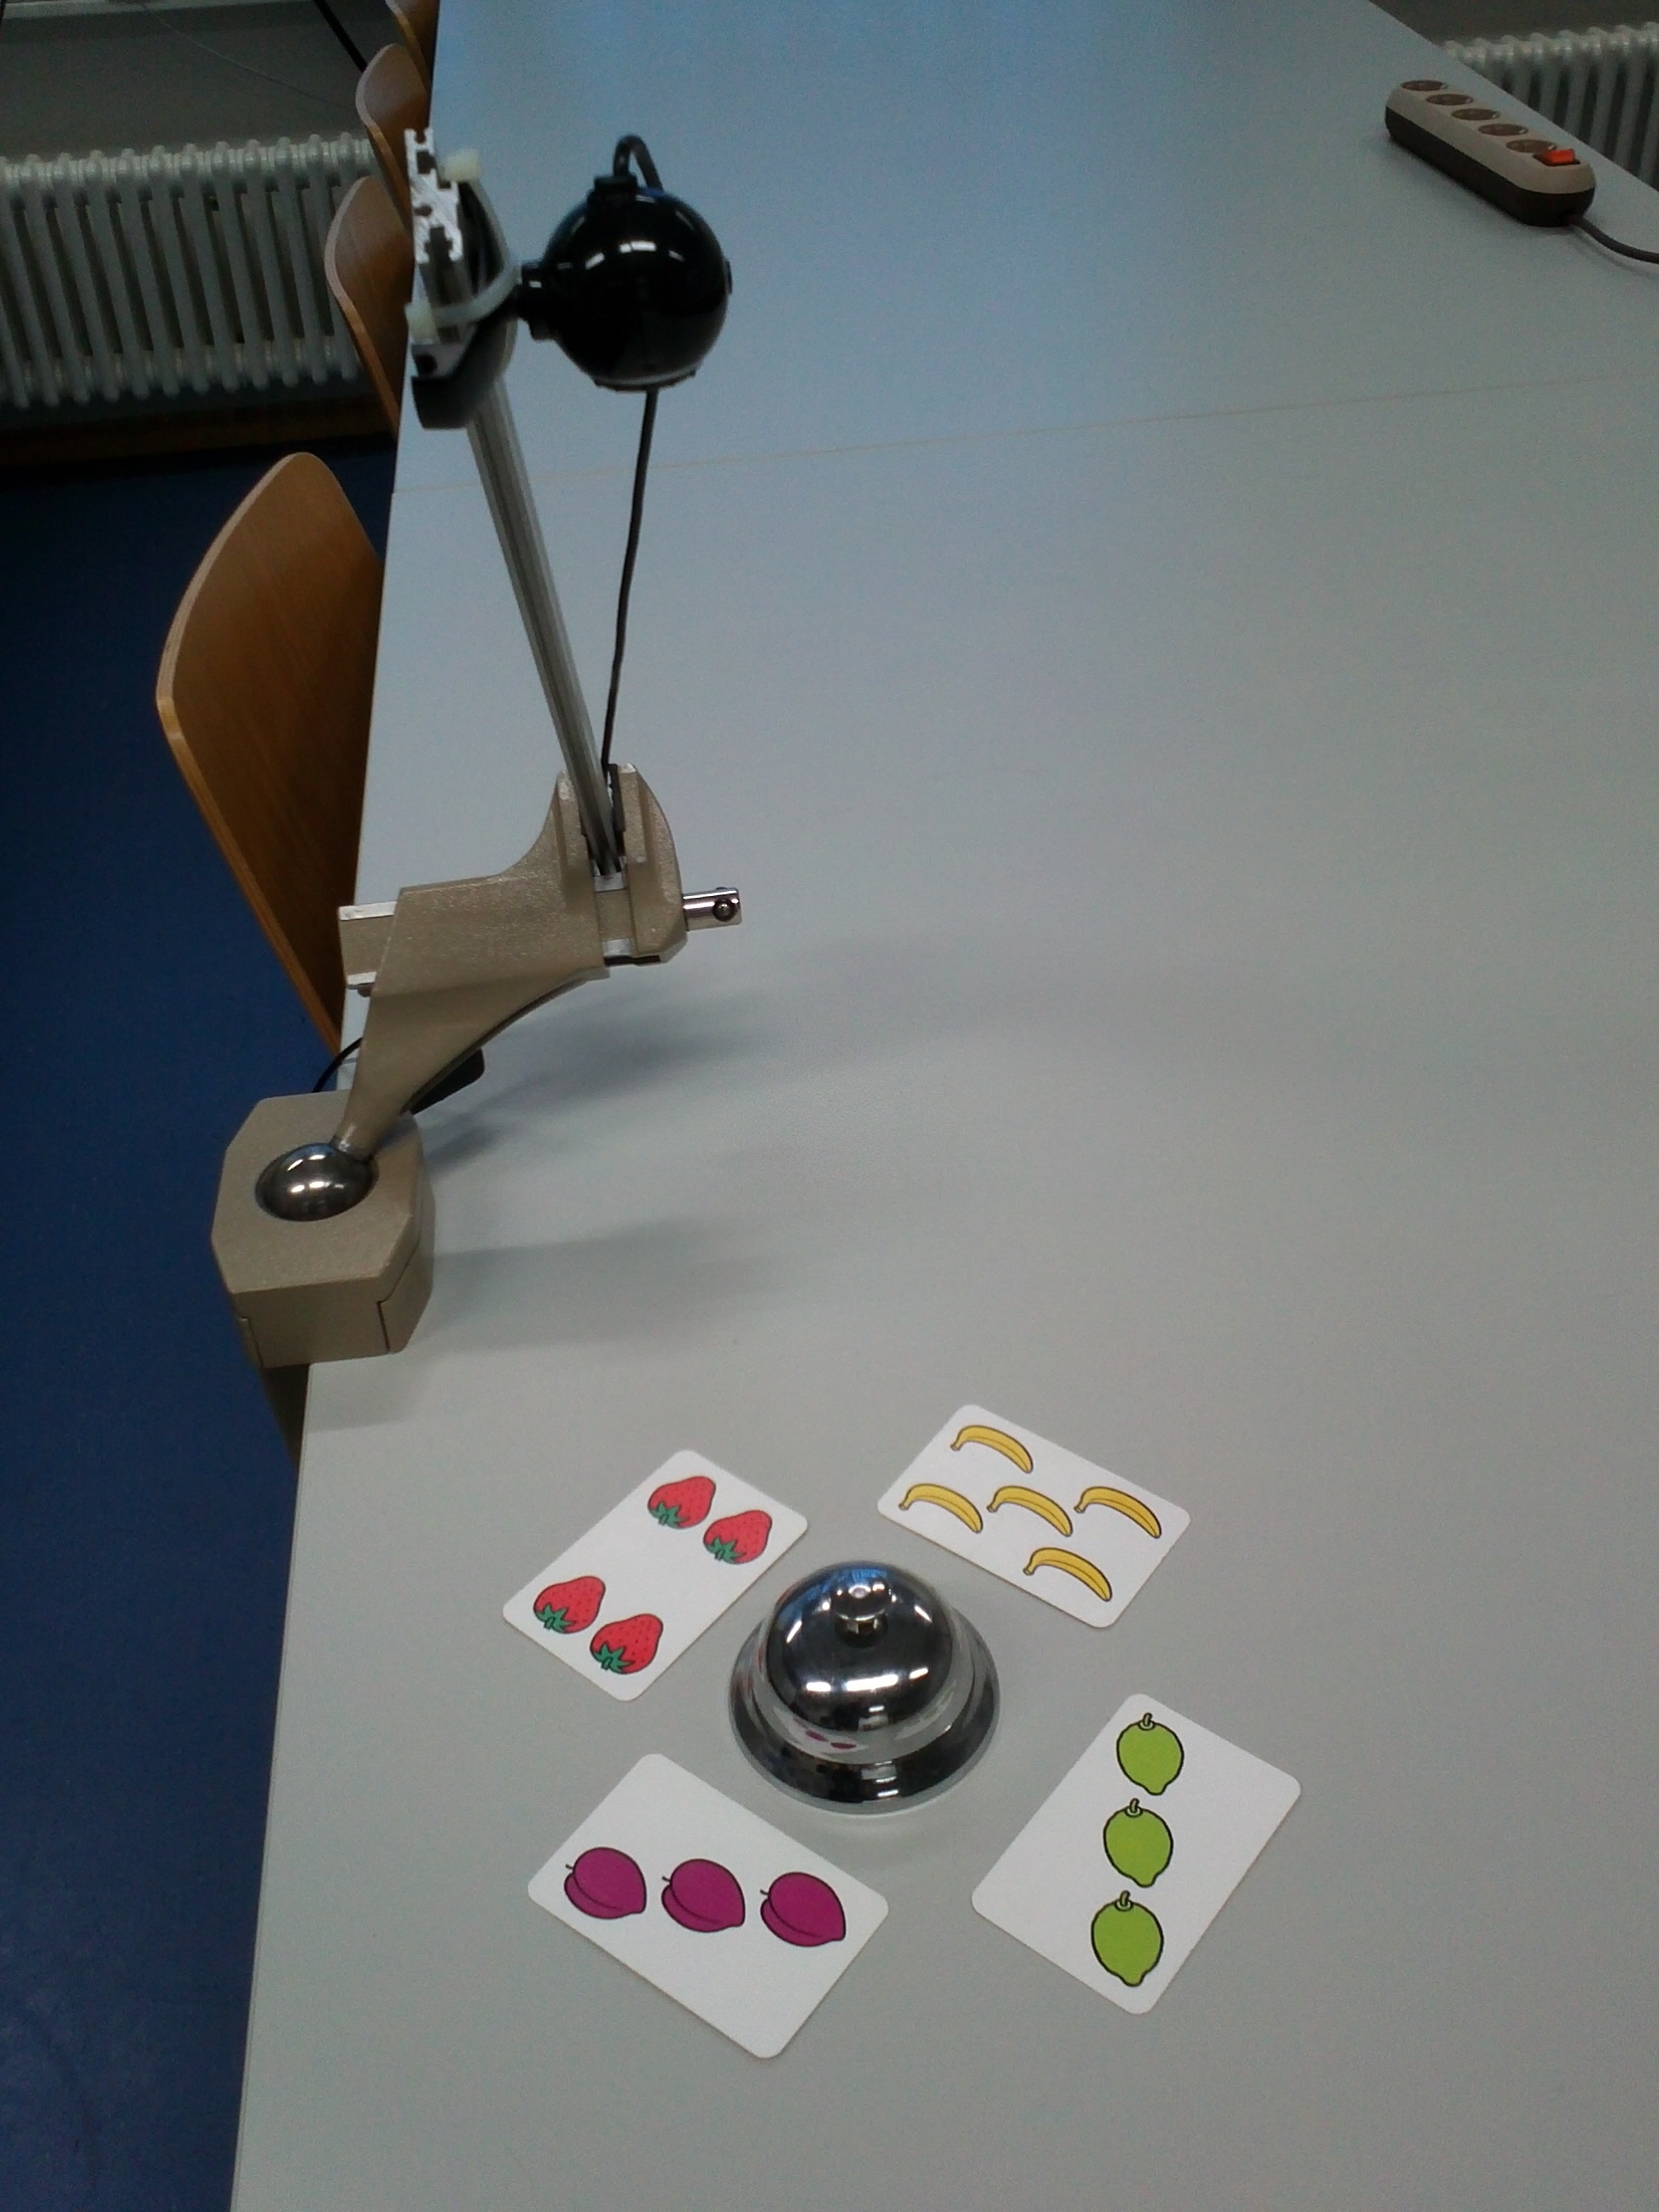
\includegraphics[width=7cm]{Abbildungen/KameraAufbau}
    \caption[Anlage]{Anlagenaufbau}
    \label{fig:Anlage}
\end{figure}

Der Spielaufbau entspricht dem original Halli Galli Aufbau mit vier Mitspielern. Abbildung~\ref{fig:Spielaufbau} zeigt die mittig positionierte Glocke, um die vier Ablagestabel der Spieler angeordnet sind.\\

%Abbildung Foto, wie die Karten liegen
\begin{figure}[h]
    \centering
    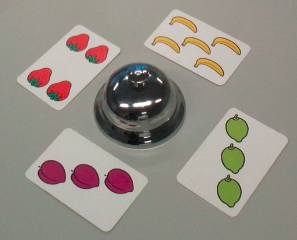
\includegraphics[width=6cm]{Abbildungen/Aufbau4}
    \caption[Spielaufbau]{Halli Galli - Spielaufbau mit vier Mitspielern}
    \label{fig:Spielaufbau}
\end{figure}


%hier sollen die vier Spielkarten (vier Früchte einzeln sein)

%\begin{center}
%\begin{tabular}{cccc}
  %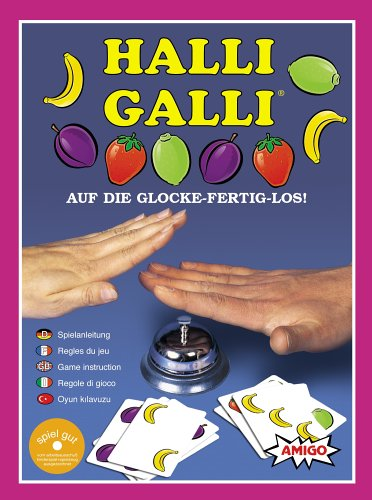
\includegraphics[width=3cm]{Abbildungen/Cover} & 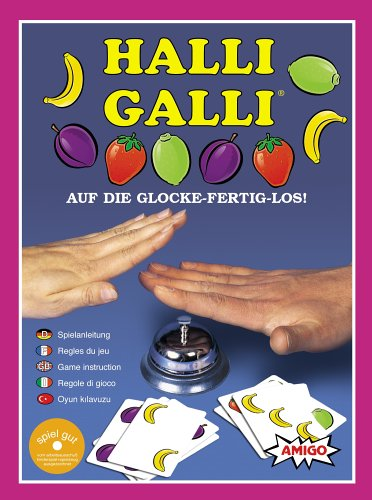
\includegraphics[width=3cm]{Abbildungen/Cover} & %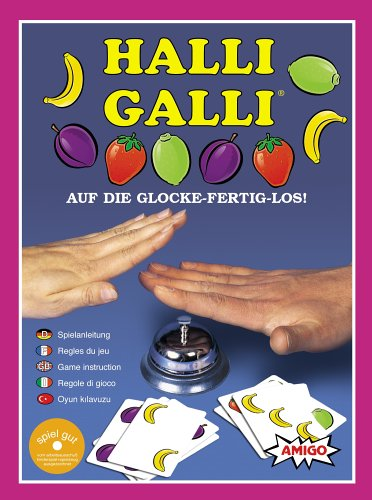
\includegraphics[width=3cm]{Abbildungen/Cover} & 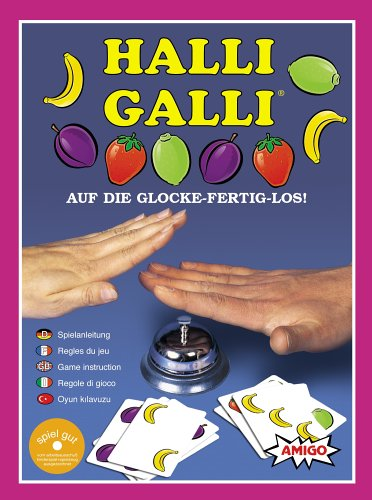
\includegraphics[width=3cm]{Abbildungen/Cover} \\ 
%\end{tabular}

%\end{center}





%1.) Theoretische Grundlagen (z.B. Messprinzip)

%2.) Genaue Beschreibung des Geräteaufbaus (Bilder)

%3.) Beschreibung der Halcon-Programmstruktur und die Funktionsweise der Programmblöcke

%4.) Gut dokumentierter Halcon-Code 

%) Ergebnisse 

%6.) Testbilder, um das Programm auch ohne Kamera testen zu können.

%Die Doku auf CD mit allen Bilder muss dem gedruckten Bericht beigelegt werden.

%BILDER:

%Jede Frucht einmal einzeln - Foto von der Karte

%Screenshot - von den schwarz / weiß Erkennung - inkl. Bild dazu 

%verschiedene Test - Bilder
